\chapter{Full AI Prompt Log}

Full prompt log được nộp dưới dạng Markdown tại \path{ai/prompt_log.md} để giữ
nguyên Unicode, code block, đường dẫn và output dài mà không làm mất cấu trúc
trong PDF. File gồm 61 interaction theo thứ tự thời gian, từ
\texttt{S001-I001} đến \texttt{S001-I061}, tổng cộng 3,801 dòng. Mỗi interaction
ghi công cụ/model, thời điểm, prompt nguyên văn, output nguyên văn và metadata
review tương ứng.

\begin{table}[H]
  \centering
  \small
  \begin{tabular}{llr}
    \toprule
    Session & Interaction & Số lượng \\
    \midrule
    S001 & I001--I017 & 17 \\
    S001 & I018--I029 & 12 \\
    S001 & I030--I036 & 7 \\
    S001 & I037--I044 & 8 \\
    S001 & I045--I061 & 17 \\
    \midrule
    Tổng & I001--I061 & 61 \\
    \bottomrule
  \end{tabular}
  \caption{Chỉ mục Full AI Prompt Log.}
  \label{tab:full-ai-log-index}
\end{table}

\textbf{SHA-256 của file log tại thời điểm xuất bản:}

\begin{center}
\small\texttt{AEB24C944CD487C16274DFDE3A5C4D4AE521B2F887D421C34CFDE5B170C9E776}
\end{center}

Bản Markdown nói trên là bản full log có thẩm quyền trong gói nộp. Bản PDF độc
lập tại \path{ai/Full_AI_Prompt_Log.pdf} được tạo từ chính file này và được nhúng
nguyên văn dưới đây, không rút gọn hoặc biên tập lại.

\clearpage
\section{Nội dung Full AI Prompt Log}

\newcount\promptlogpage
\promptlogpage=1
\loop
  \clearpage
  \thispagestyle{plain}
  \begin{center}
    \includegraphics[
      page=\the\promptlogpage,
      width=\textwidth,
      height=0.91\textheight,
      keepaspectratio
    ]{../../ai/Full_AI_Prompt_Log.pdf}
  \end{center}
  \advance\promptlogpage by 1
\ifnum\promptlogpage<69
\repeat
